\documentclass[border=3pt]{standalone}
\usepackage{tikz}
\usetikzlibrary{arrows.meta,calc}
\tikzset{pin/.style={-{Stealth[length=5pt]}},
  blk/.style={draw, thick, minimum width=22mm, minimum height=28mm, font=\sffamily\small, align=center}}
\begin{document}
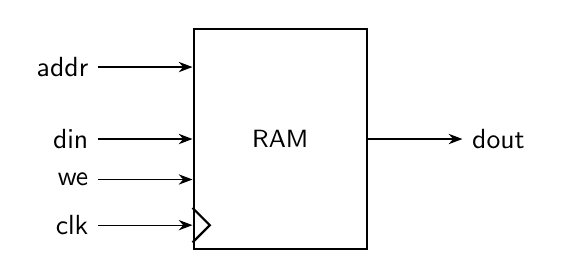
\begin{tikzpicture}[font=\sffamily]
  \node[blk] (m) {RAM};
  \draw[thick] ($(m.south west)+(0,1mm)$) -- ++(2.2mm,2.2mm) -- ++(-2.2mm,2.2mm);
  \draw[pin] ($(m.north west)+(-12mm,-5mm)$) node[left]{addr} -- ($(m.north west)+(0,-5mm)$);
  \draw[pin] ($(m.west)+(-12mm,0)$) node[left]{din} -- (m.west);
  \draw[pin] ($(m.south west)+(-12mm,9mm)$) node[left]{we} -- ($(m.south west)+(0,9mm)$);
  \draw[pin] ($(m.east)+(0,0)$) -- ++(12mm,0) node[right]{dout};
  \draw[pin] ($(m.south west)+(-12mm,3.2mm)$) node[left]{clk} -- ($(m.south west)+(0,3.2mm)$);
\end{tikzpicture}
\end{document}
